
\section{ Flex Layout }

\subsection{ What is Flex Layout }
Flex layout provies an HTML UI layout for Angular applications; using Flexbox
and a Responsive API.

\subsection{ Understanding the Issue With CSS Based Flexbox }
\begin{itemize}
  \item CSS specifity \footnote{CSS speicifity, is the means by which browsers
  decide which CSS property values are the most relevant to an element and,
  therefore, will be applied} issues rapidly become problemtic, and continue
  to be so.
  \item CSS footprint size becomes excessively large(>250k for flexbox CSS)
  whereas with JS, the module is loaded within every specific module
  \item Changes in layout direction required changes to child flexbox stylings
  \item No built in support for customized media query breakpoints (need to 
  specify them yourself)
\end{itemize}

\subsection{ Why Use Flex Layout? }
\begin{itemize}
  \item Flex Layout is indexpendent of Angular material
  \item No external Css requirements
  \item Support for Handeset/Tablet and Orientation breakpoints
  \item Support for any layour injector value
  \item Support for raw values, or interpolated values
  \item Support for raw, percentage, or px-suffix values. Change detection
  for Layout injector values.
  \item Use provider to supply custom breakpoints
  \item Notifications for breakpoints changes
  \item MediaQuery Activation detection
\end{itemize}

\subsection{ A Great Example of Flex Layout }

One of the greatest selling points with regards to flex layout, is that it makes
responsive design very easy to do. In particular, it's ability to apply a gap
between elements, and easily change them between different devices. However, I
would like to show an example of the piece of code that sold me on flex layout.
I was playing around with a feature called fxLayoutGap. It particular, it uses
margin-right used when the parent container \lstinline{flex-direction == "row"}
and margin-bottom is used when the parent container \lstinline{flex-direction == "column"}

So for instance, let's say we have a div will be using flex. We would like
there to be two divs inside, with a margin-left of 16px. This is how we would
do it if we weren't using fxLayoutGap.
\begin{lstlisting}
.icon-text {
  margin-left: mc-space-multiplier(1);
}
.section {
  margin-top: mc-space-multiplier(4);
}
\end{lstlisting}


The following is a great example, of what can be done with flex-layout.


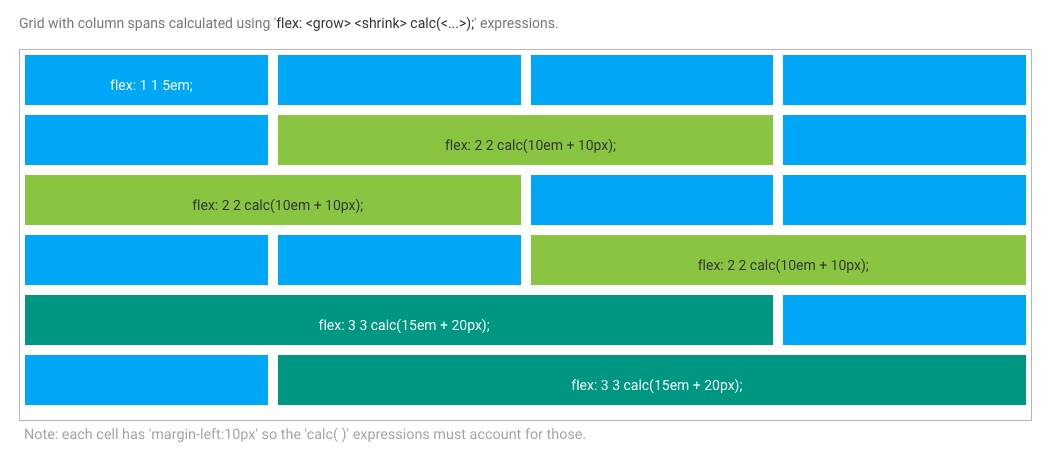
\includegraphics[width=9.1cm, height=6cm]{pwa/responsive/flex-layout/flex-layout-grid}
The following is the code which produces the above:


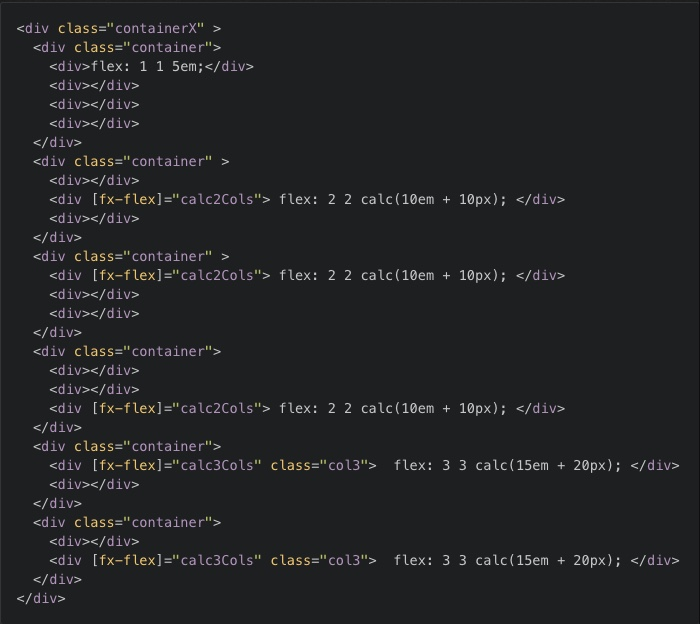
\includegraphics[width=9.1cm, height=6cm]{pwa/responsive/flex-layout/flex-layout-code}
